\documentclass[12pt,border=12pt]{standalone}
\usepackage[utf8]{inputenc}
\usepackage{tikz}
\usepackage{lmodern}
\usepackage{amsmath,amssymb}
\usetikzlibrary{shapes.geometric,arrows.meta,positioning,calc,fit,backgrounds,shadows}

\begin{document}
\fontsize{12pt}{15pt}\selectfont

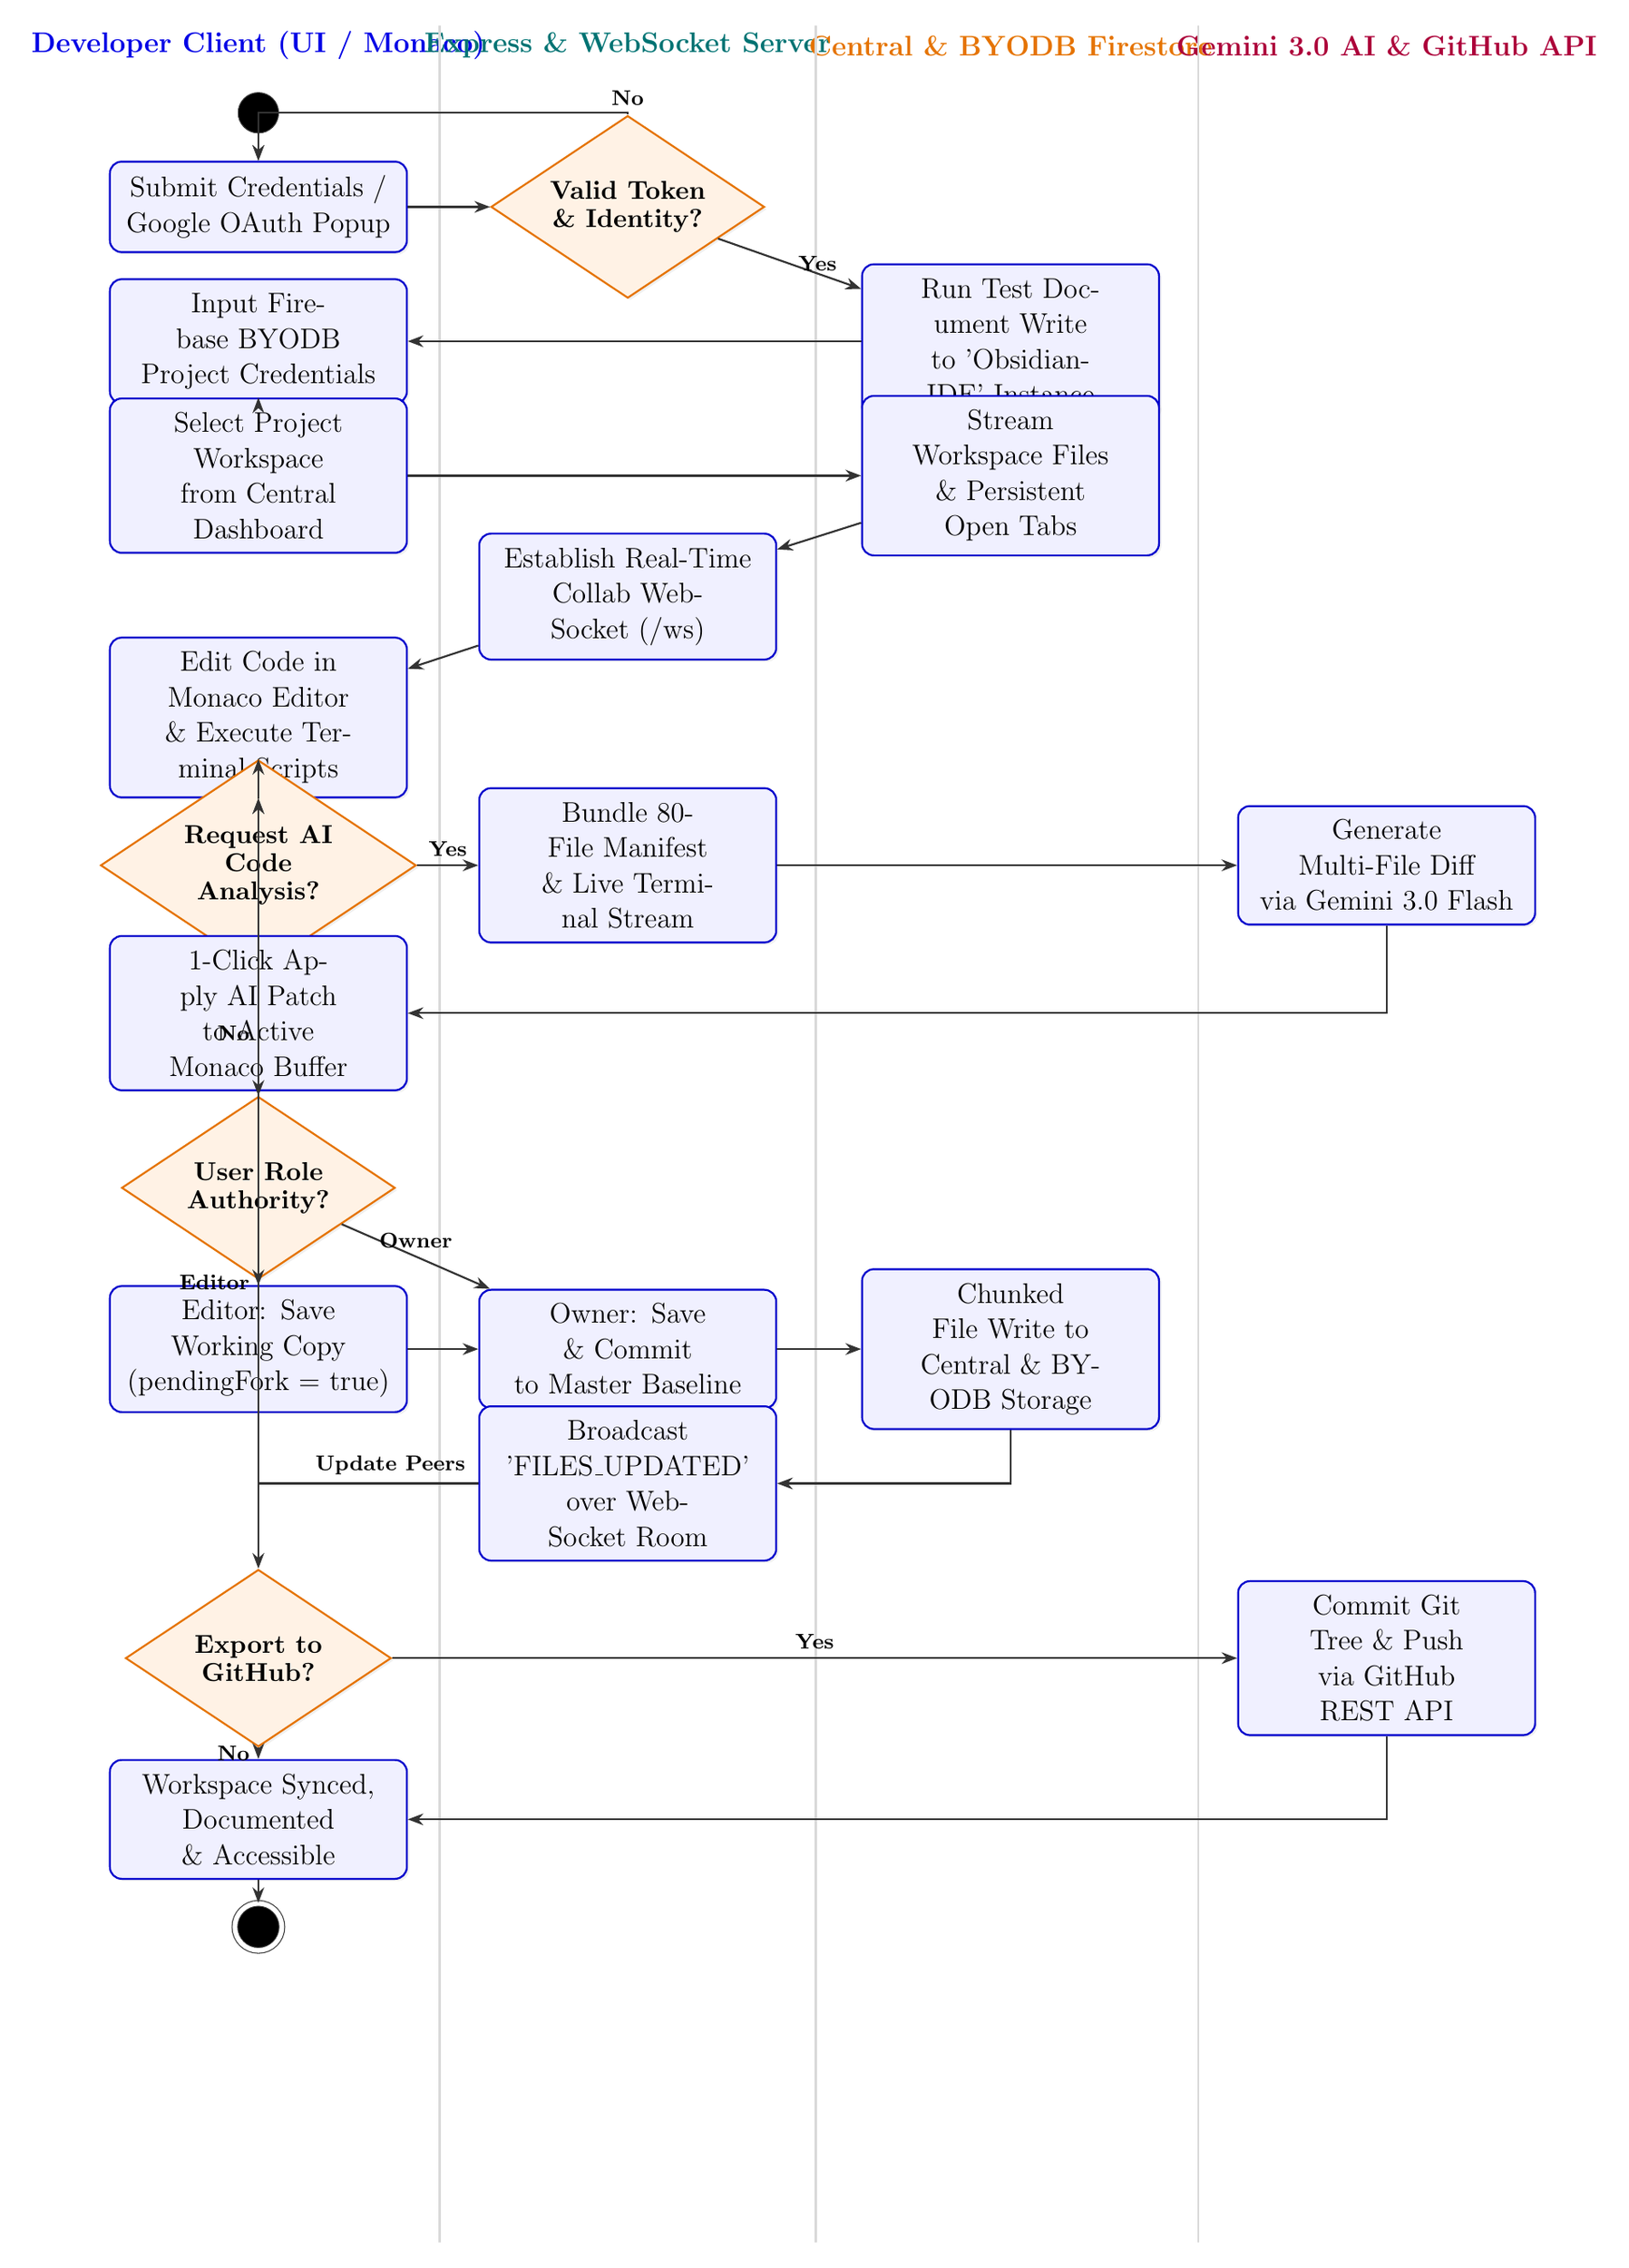
\begin{tikzpicture}[
    font=\fontsize{12pt}{15pt}\selectfont,
    >=Stealth,
    activity/.style={
        rectangle,
        draw=blue!80!black,
        fill=blue!6!white,
        thick,
        rounded corners=5pt,
        align=center,
        inner sep=6pt,
        text width=4.0cm,
        minimum height=1.0cm,
        drop shadow={opacity=0.12,shadow xshift=1pt,shadow yshift=-1pt}
    },
    decision/.style={
        diamond,
        draw=orange!90!black,
        fill=orange!10!white,
        thick,
        align=center,
        inner sep=3pt,
        aspect=1.5,
        text width=2.4cm,
        font=\fontsize{10.5pt}{12pt}\selectfont\bfseries,
        drop shadow={opacity=0.12,shadow xshift=1pt,shadow yshift=-1pt}
    },
    startStop/.style={
        circle,
        draw=black!80,
        fill=black,
        inner sep=0pt,
        minimum size=0.6cm
    },
    endCircle/.style={
        circle,
        draw=black!80,
        double=white,
        double distance=2pt,
        fill=black,
        inner sep=0pt,
        minimum size=0.7cm
    },
    forkBar/.style={
        rectangle,
        fill=black!80,
        minimum width=4.2cm,
        minimum height=0.15cm,
        rounded corners=1pt
    },
    flowLine/.style={
        thick,
        draw=black!80,
        ->
    },
    laneBox/.style={
        draw=gray!40,
        fill=gray!2!white,
        dashed,
        rounded corners=6pt
    }
]

% ==================== SWIMLANE HEADERS ====================
\node[font=\bfseries\large, text=blue!90!black] at (-7.0, 13.2) {Developer Client (UI / Monaco)};
\node[font=\bfseries\large, text=teal!90!black] at (-1.5, 13.2) {Express \& WebSocket Server};
\node[font=\bfseries\large, text=orange!90!black] at (4.2, 13.2) {Central \& BYODB Firestore};
\node[font=\bfseries\large, text=purple!90!black] at (9.8, 13.2) {Gemini 3.0 AI \& GitHub API};

\draw[gray!30, thick] (-4.3, 13.5) -- (-4.3, -19.5);
\draw[gray!30, thick] (1.3, 13.5) -- (1.3, -19.5);
\draw[gray!30, thick] (7.0, 13.5) -- (7.0, -19.5);

% ==================== STEP 1: AUTH & ONBOARDING ====================
\node[startStop] (startNode) at (-7.0, 12.2) {};
\node[activity] (actLogin) at (-7.0, 10.8) {Submit Credentials /\\Google OAuth Popup};
\node[decision] (decAuth) at (-1.5, 10.8) {Valid Token\\\& Identity?};
\node[activity] (actOnboard) at (-7.0, 8.8) {Input Firebase BYODB\\Project Credentials};
\node[activity] (actVerifyBYODB) at (4.2, 8.8) {Run Test Document Write\\to 'ObsidianIDE' Instance};

\draw[flowLine] (startNode) -- (actLogin);
\draw[flowLine] (actLogin) -- (decAuth);
\draw[flowLine] (decAuth) -- node[above, font=\small\bfseries] {No} ++(0, 1.4) -| (actLogin);
\draw[flowLine] (decAuth) -- node[right, font=\small\bfseries] {Yes} (actVerifyBYODB);
\draw[flowLine] (actVerifyBYODB) -- (actOnboard);

% ==================== STEP 2: WORKSPACE & MONACO ====================
\node[activity] (actOpenWS) at (-7.0, 6.8) {Select Project Workspace\\from Central Dashboard};
\node[activity] (actLoadManifest) at (4.2, 6.8) {Stream Workspace Files\\\& Persistent Open Tabs};
\node[activity] (actWSConnect) at (-1.5, 5.0) {Establish Real-Time\\Collab WebSocket (/ws)};

\draw[flowLine] (actOnboard) -- (actOpenWS);
\draw[flowLine] (actOpenWS) -- (actLoadManifest);
\draw[flowLine] (actLoadManifest) -- (actWSConnect);

% ==================== STEP 3: CODE EDITING & AI ====================
\node[activity] (actMonacoEdit) at (-7.0, 3.2) {Edit Code in Monaco Editor\\\& Execute Terminal Scripts};
\node[decision] (decAI) at (-7.0, 1.0) {Request AI\\Code Analysis?};
\node[activity] (actPromptAI) at (-1.5, 1.0) {Bundle 80-File Manifest\\\& Live Terminal Stream};
\node[activity] (actGeminiInfer) at (9.8, 1.0) {Generate Multi-File Diff\\via Gemini 3.0 Flash};
\node[activity] (actApplyPatch) at (-7.0, -1.2) {1-Click Apply AI Patch\\to Active Monaco Buffer};

\draw[flowLine] (actWSConnect) -- (actMonacoEdit);
\draw[flowLine] (actMonacoEdit) -- (decAI);
\draw[flowLine] (decAI) -- node[above, font=\small\bfseries] {Yes} (actPromptAI);
\draw[flowLine] (actPromptAI) -- (actGeminiInfer);
\draw[flowLine] (actGeminiInfer) |- (actApplyPatch);
\draw[flowLine] (actApplyPatch) -- (actMonacoEdit);

% ==================== STEP 4: ROLE-BASED SYNC ====================
\node[decision] (decRole) at (-7.0, -3.8) {User Role\\Authority?};
\node[activity] (actSaveFork) at (-7.0, -6.2) {Editor: Save Working Copy\\(pendingFork = true)};
\node[activity] (actOwnerSync) at (-1.5, -6.2) {Owner: Save \& Commit\\to Master Baseline};
\node[activity] (actPersistCloud) at (4.2, -6.2) {Chunked File Write to\\Central \& BYODB Storage};
\node[activity] (actBroadcastWS) at (-1.5, -8.2) {Broadcast 'FILES\_UPDATED'\\over WebSocket Room};

\draw[flowLine] (decAI) -- node[left, font=\small\bfseries] {No} (decRole);
\draw[flowLine] (decRole) -- node[left, font=\small\bfseries] {Editor} (actSaveFork);
\draw[flowLine] (decRole) -- node[above, font=\small\bfseries] {Owner} (actOwnerSync);
\draw[flowLine] (actSaveFork) -- (actOwnerSync);
\draw[flowLine] (actOwnerSync) -- (actPersistCloud);
\draw[flowLine] (actPersistCloud) |- (actBroadcastWS);
\draw[flowLine] (actBroadcastWS) -| node[above, font=\small\bfseries, pos=0.2] {Update Peers} (actMonacoEdit);

% ==================== STEP 5: GITHUB EXPORT & END ====================
\node[decision] (decGH) at (-7.0, -10.8) {Export to\\GitHub?};
\node[activity] (actGHExport) at (9.8, -10.8) {Commit Git Tree \& Push\\via GitHub REST API};
\node[activity] (actComplete) at (-7.0, -13.2) {Workspace Synced,\\Documented \& Accessible};
\node[endCircle] (endNode) at (-7.0, -14.8) {};

\draw[flowLine] (actSaveFork) -- (decGH);
\draw[flowLine] (decGH) -- node[above, font=\small\bfseries] {Yes} (actGHExport);
\draw[flowLine] (actGHExport) |- (actComplete);
\draw[flowLine] (decGH) -- node[left, font=\small\bfseries] {No} (actComplete);
\draw[flowLine] (actComplete) -- (endNode);

\end{tikzpicture}
\end{document}
